
\chapter{Exploring Clustering Pipelines via AutoML and Diversificationg}
\label{data-centric-chap:unsupervised}

\begin{figure}[t]
    \begin{subfigure}[t]{0.23\columnwidth}
        \centering
        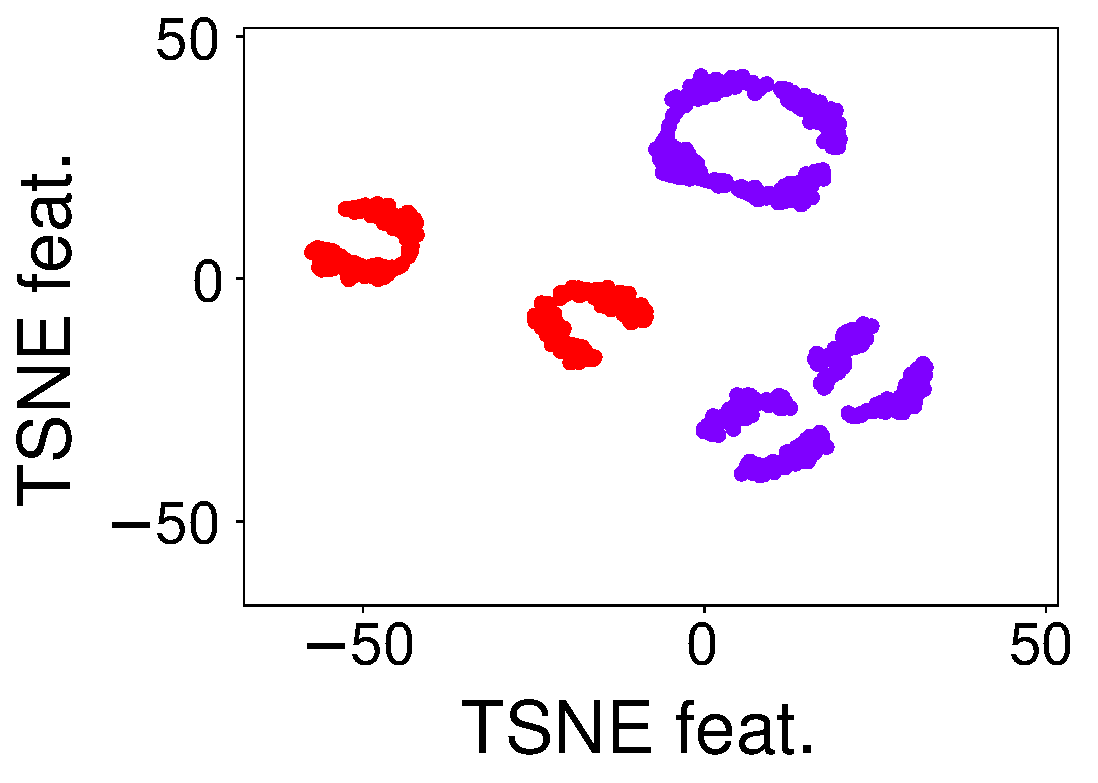
\includegraphics[scale=.15]{chapters/data-centric/unsupervised/img/cl.pdf}
        \caption{Cl \cite{Tschechlov2021}\\ \scriptsize{AMI=0.41, sil=0.41}}
        \label{clustering-fig:ca3}
    \end{subfigure}
    ~
    \begin{subfigure}[t]{0.23\columnwidth}
        \centering
        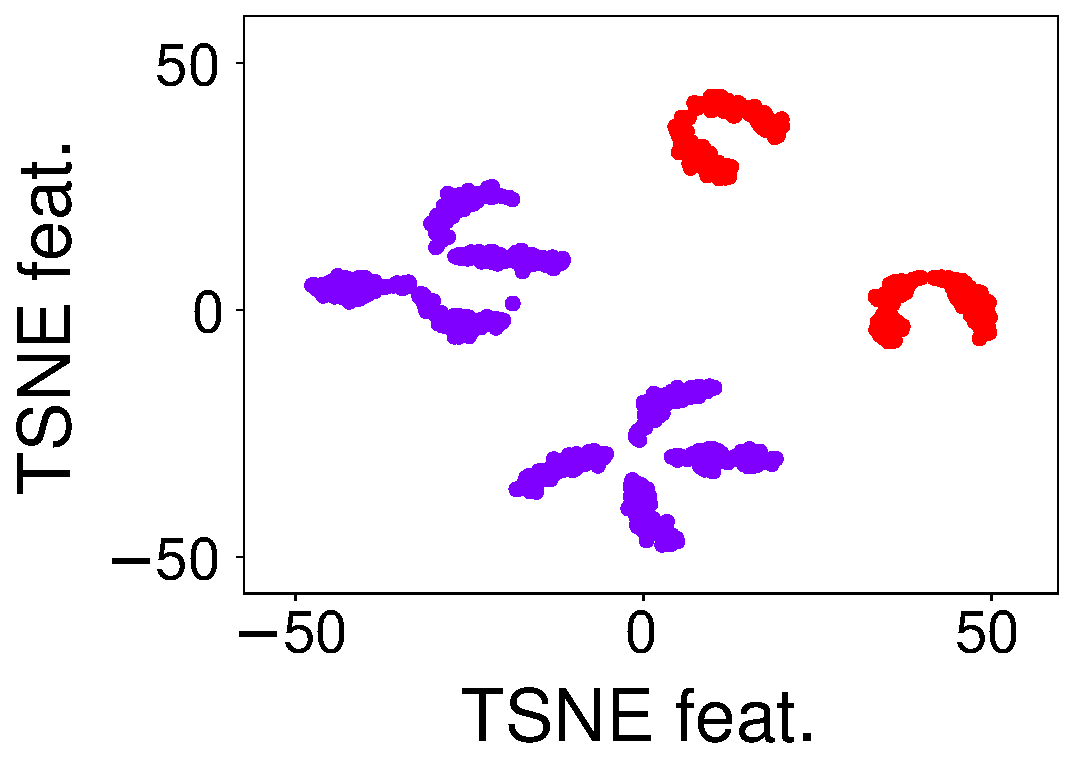
\includegraphics[scale=.15]{chapters/data-centric/unsupervised/img/ft_cl.pdf}
        \caption{FS + Cl\\ \scriptsize{AMI=0.41, sil=0.47}}
        \label{clustering-fig:ca4}
    \end{subfigure}
    ~
    \begin{subfigure}[t]{0.2\columnwidth}
        \centering
        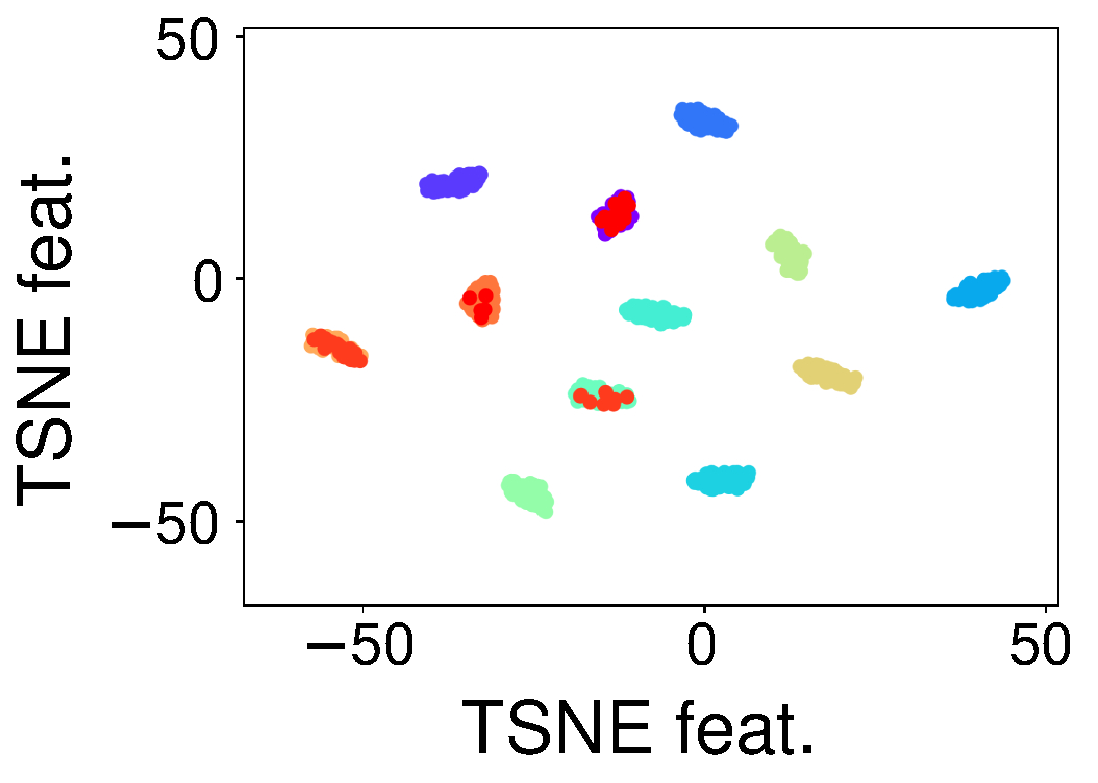
\includegraphics[scale=.15]{chapters/data-centric/unsupervised/img/ft_sc_cl.pdf}
        \caption{FS + N + Cl\\ \scriptsize{AMI=0.9, sil=0.87}}
        \label{clustering-fig:ca5}
    \end{subfigure}
    ~
    \begin{subfigure}[t]{0.28\columnwidth}
        \centering
        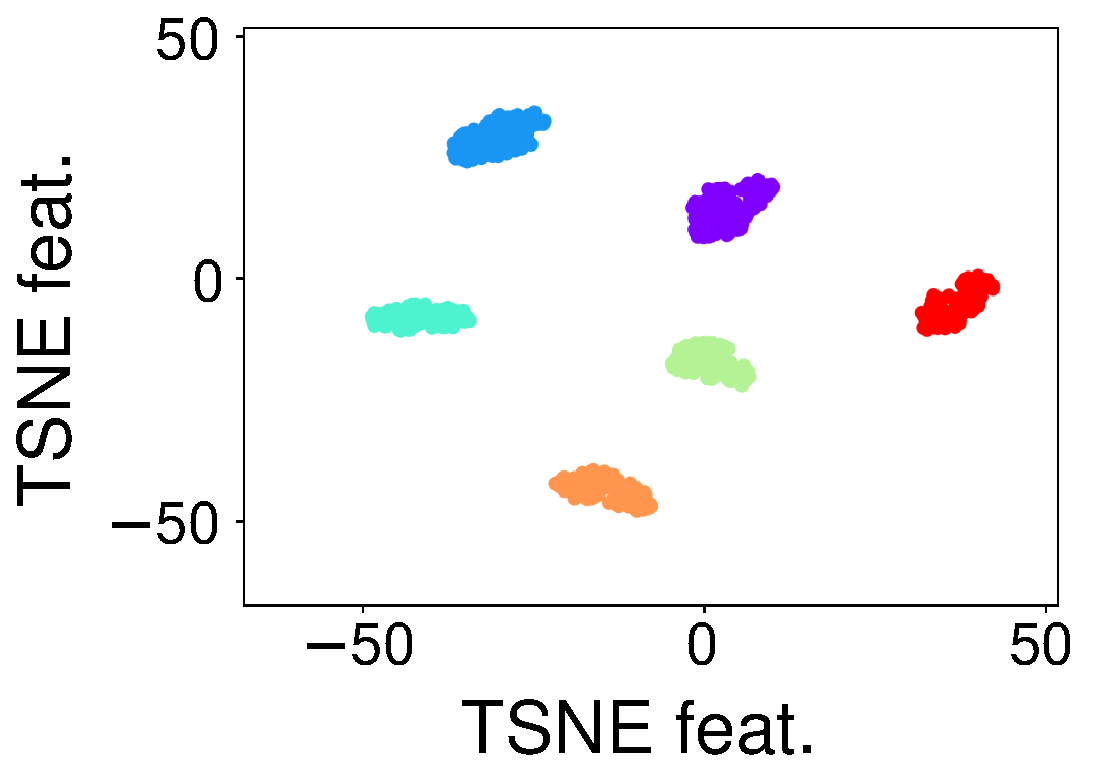
\includegraphics[scale=.15]{chapters/data-centric/unsupervised/img/ft_sc_ou_cl.pdf}
        \caption{FS + N + OR + Cl\\ \scriptsize{AMI=1.0, sil=0.92}}
        \label{clustering-fig:ca6}
    \end{subfigure}
    \caption{Approach motivation. \\
    \small{Feature Selection (FS) - Normalization (N) - Outlier Removal (OR) - Clustering (Cl)}}
    \label{clustering-fig:clusterings}
\end{figure}

% Thanks to the abundant presence of data, machine learning (ML) has been employed in a variety of fields (e.g., urban mobility \cite{toch2019analyzing}).
% Depending on the scope of the analysis, the task is defined either supervised (i.e., leveraging a ground truth; e.g., classification) or unsupervised (i.e., without ground truth; e.g., cluster analysis).
% Data scientists design the workflow as a \textit{ML pipeline}; namely, a series of pre-processing steps (e.g., features selection) are in charge of shaping the data so that the final analysis step can produce the best result.
% For each step of the pipeline, there are alternative algorithms (e.g., SPEC \cite{zhao2007spectral} for feature selection, KMeans \cite{arthur2006k} for cluster analysis), each with hyperparameters to tune (e.g., the number of features or clusters, respectively).

% It is well known that, given the exponential search space, the tuning process is tedious and overwhelming.
\textit{Automated Machine Learning} aids in a smart exploration of the hyperparameter search space \cite{hutter2011sequential} and lets data scientists focus on analyzing and interpreting the extracted results.
AutoML has been proven to be effective on supervised tasks where the ground truth eases the evaluation of the hyperparameters optimality   \cite{thornton2013auto,FRANCIA2023182}; yet, when it comes to unsupervised tasks, the road is not paved yet \cite{barlow1989unsupervised}.
In this chapter, we focus on the unsupervised task of \textit{(crisp) cluster analysis} \cite{arthur2006k} that returns a partitioning of the original dataset based on the similarity of data items.
Cluster analysis is exploratory by nature since, given that no ground truth is available, there is no ``correct'' result \cite{no_correct_clustering,lensen2017using} and the aim for the data scientist is to uncover clues hidden in the data.
\paragraph{Challenges} The two main limitations of the AutoML approaches in the literature are (i) auto-tuning is applied to the ML step only, disregarding the pre-processing ones, and (ii) only the most-performing pipeline configuration is returned; although this is reasonable in the supervised context, it provides limited information in unsupervised one due the exploratory nature of the analysis.

\paragraph{Contributions} To overcome the previous limitations, we devise AutoClues: an \textit{end-to-end} AutoML approach that provides a \textit{dashboard} of \textit{relevant} and \textit{different} clusterings. In particular, we focus on the following contributions:
\begin{itemize}
    \item \textit{generalizing} AutoML formulation to unsupervised tasks dealing with ML pipelines;
    \item \textit{tuning} a thorough ML pipeline to discover clusterings that would have been unrevealed otherwise;
    \item \textit{diversifying} the generated clusterings to ensure that the dashboard is both high-quality and leads to different insights (i.e., disclose something new);
    \item \textit{providing} a customizable generator of synthetic datasets for benchmarking in (crisp) cluster analysis.
\end{itemize}

To let the reader appreciate the novelty of AutoClues, we rely on a synthetic 10-dimensional (10D) dataset that includes 6 natural clusters. \Cref{clustering-fig:ca3} shows the t-SNE \cite{van2008visualizing} visualization\footnote{Clusterings in more than two dimensions will be always visualized in 2D applying the t-SNE dimensionality reduction.}  of the clustering obtained applying AutoML4Clust \cite{Tschechlov2021}, an approach of the literature, that solely tunes the clustering step $Cl$. \Cref{clustering-fig:ca4,fig:ca5,fig:ca6} show the clusterings obtained by tuning an ML pipeline that incrementally includes feature selection ($FS$), normalization ($N$), and outlier removal ($OR$). In (b), $FS$ identifies the most relevant features; in (c), $N$ standardizes such features thus avoiding bias due to different domain ranges; in (d), $OR$ drops any data items that are not representative. 
It is apparent how the tuning improves throughout the different steps, making it possible for $Cl$ to properly detect the 6 natural clusters. 
To quantitatively understand the improvements, we rely on the silhouette index $sil \in [-1, 1]$ (the higher the better), an estimation of the ``goodness'' of a clustering considering solely the data itself; namely, the \textit{separability} between the clusters and their \textit{cohesion} \cite{zhu2010clustering}.
While in real-case unsupervised problems the ground truth is not available, for our synthetic example we can also measure how the returned clusters match the synthetic ones through the adjusted mutual information \cite{vinh2009information} $AMI \in [0, 1]$ (the higher the better).

\begin{figure}[t]  
    \begin{subfigure}[t]{0.31\columnwidth}
        \centering
        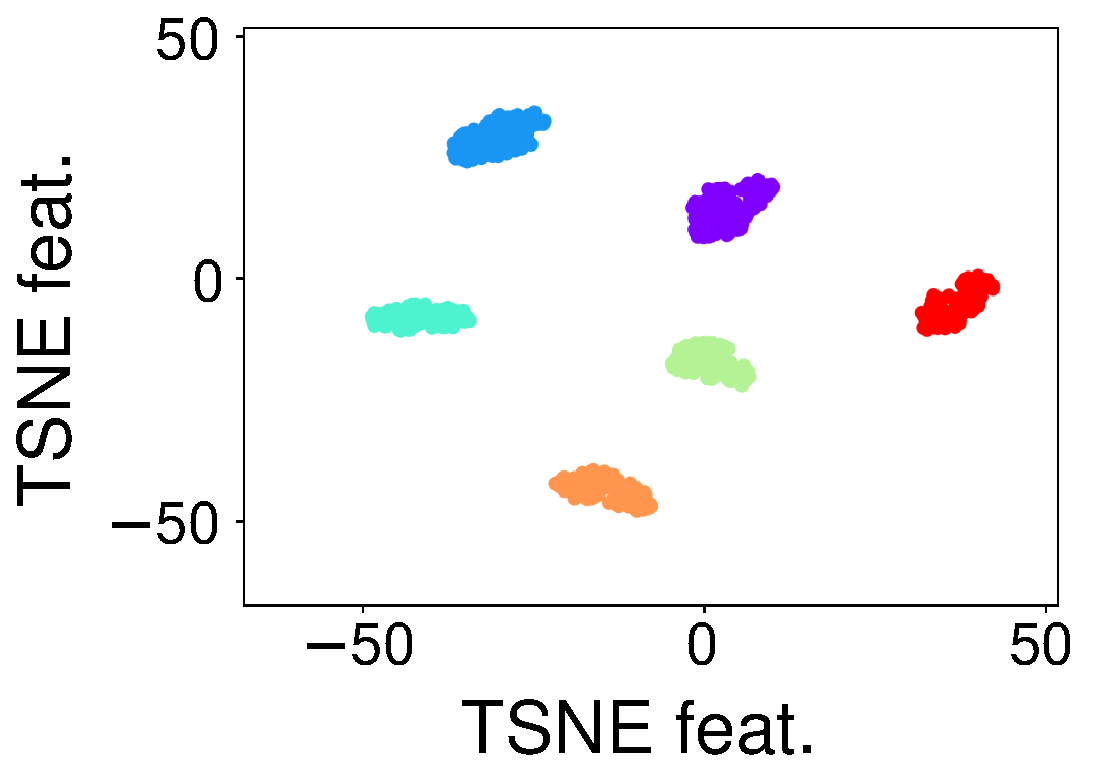
\includegraphics[scale=.15]{chapters/data-centric/unsupervised/img/ft_sc_ou_cl.pdf}
        \caption{FS + N + OR + Cl\\ \scriptsize{AMI=1.0, sil=0.92}}
        \label{clustering-fig:d1}
    \end{subfigure}
    ~~
    \begin{subfigure}[t]{0.31\columnwidth}
        \centering
        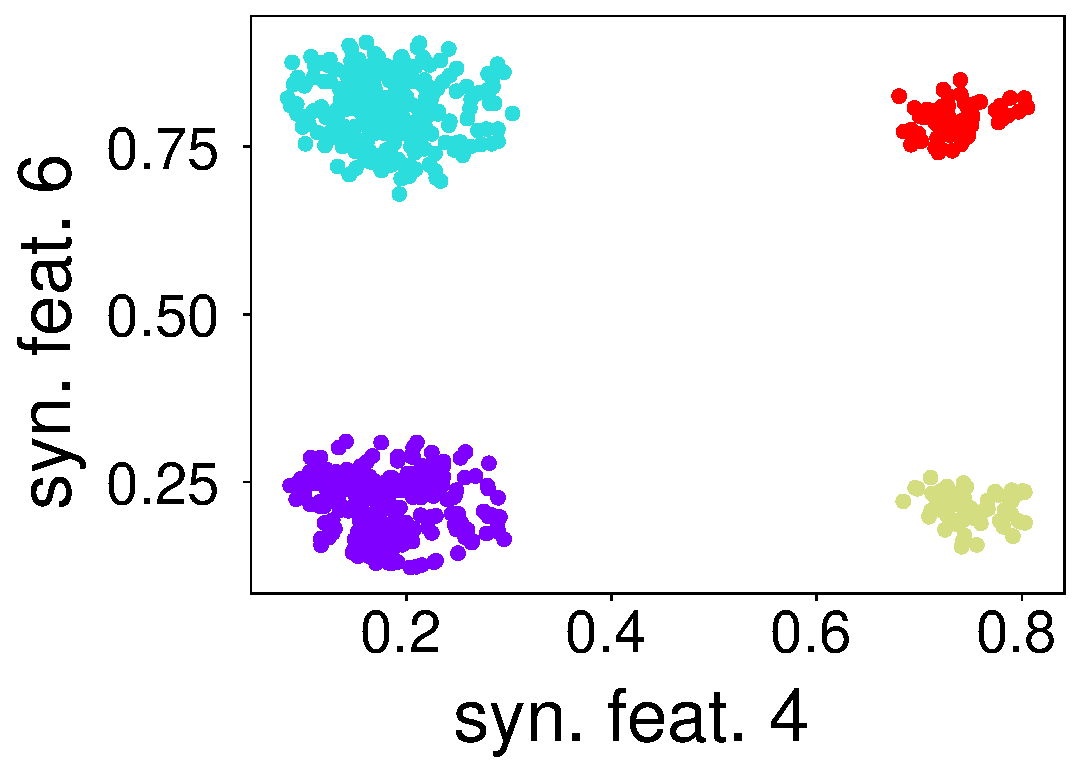
\includegraphics[scale=.15]{chapters/data-centric/unsupervised/img/dashboard_1_pred.pdf}      
        \caption{FS + OR + Cl\\ \scriptsize{AMI=0.65, sil=0.86}}
        \label{clustering-fig:d3}
    \end{subfigure}
    ~
    \begin{subfigure}[t]{0.31\columnwidth}
        \centering
        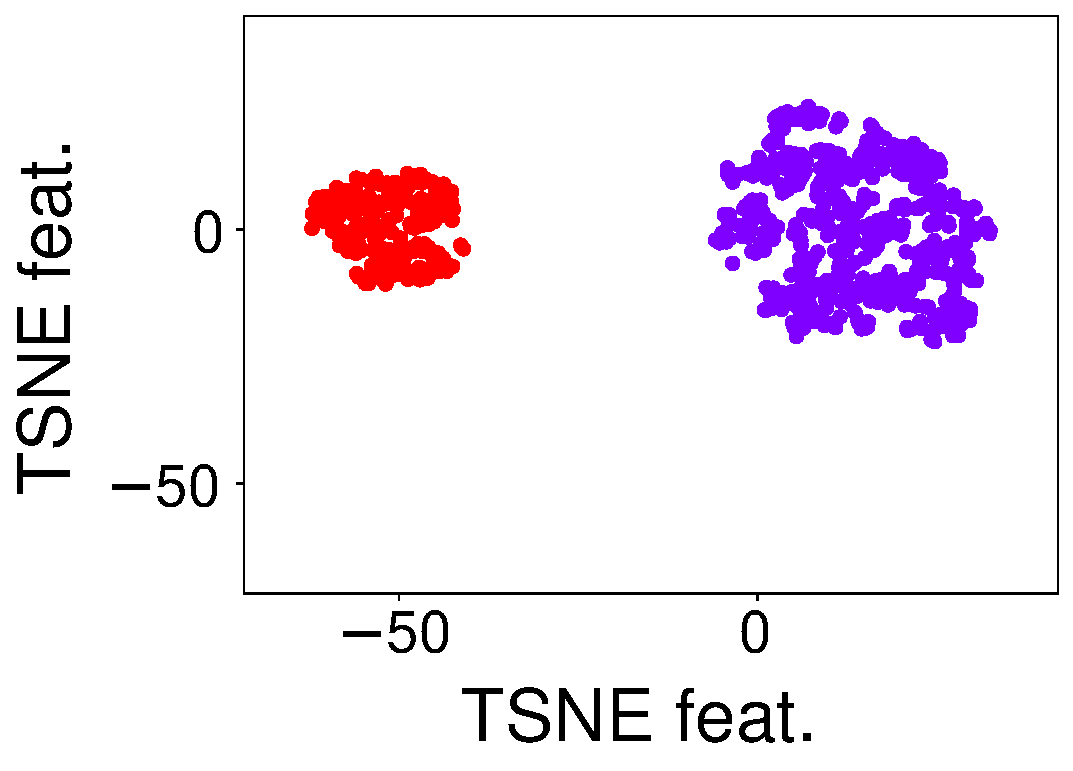
\includegraphics[scale=.15]{chapters/data-centric/unsupervised/img/dashboard_2_pred.pdf}  
        \caption{FS + OR + Cl\\ \scriptsize{AMI=0.38, sil=0.74}}
        \label{clustering-fig:d2}
    \end{subfigure}
    \caption{Relevant and diverse clusterings returned by AutoClues.\\
    \small{Feature Selection (FS) - Normalization (N) - Outlier Removal (OR) - Clustering (Cl)}}
    \label{clustering-fig:dashboard}
\end{figure}

As to the limitation of returning only the most-performing pipeline configuration, \Cref{clustering-fig:dashboard} depicts an example of an AutoClues dashboard with three different facets (clustering).
Along with the expected clusters (a), the representation in (b) unveils 4 macro clusters in 2 original features, while the representation in (c) highlights a large gap of 2 main clusters.
In real-world problems, those facets may help the data scientist to understand the data by providing different interpretations of their semantics.

We organize this chapter as follows.
\Cref{clustering-sec:related} discusses the related works; \Cref{clustering-sec:autoclues} introduces the problem formulation and how AutoClues tackles it; \Cref{clustering-sec:test} illustrates the benchmark generator and dives into the empirical evaluation of the approach; finally, \Cref{clustering-sec:conclusion} draws the conclusion and future research directions.

%\vspace{-0.2cm}
\section{Related Works}\label{clustering-sec:related}

Although the active development of data pre-processing techniques in cluster analysis (e.g., outlier removal, feature selection), and the evidence of their benefits, there is no trace of automatic solutions that tunes a thorough ML pipeline.

Former approaches employed model-free techniques (i.e., without a model to drive the optimization) to tune the combination of number of clusters and number of features.
Evolutionary algorithms are population-based heuristics inspired by biological evolution mechanisms (e.g., reproduction, mutation) or physical phenomena (e.g., particle swarm, black holes).
The population is intended as the search space, individuals are configurations, and a mutation mechanism allows the modification of the current candidate, hence the exploration.
Recent works that follow this modus operandi (i.e., MOGA \cite{dutta2013}, MODE-cf \cite{hancer2020new}) compose the candidate with a string that encodes information about both the feature selection and the clustering.
Authors in \cite{simulate_annealing} leverage simulate annealing, an algorithm that comes from a technique involving heating and controlled cooling of material in metallurgy.
In \cite{prakash2019gravitational}, it is leveraged a gravitational search algorithm, inspired by the theory of Newtonian gravity.

Model-based techniques leverage past evaluations to fit a model and visit the most prominent configurations.
Such techniques have been proven to achieve extremely good results, specifically in the (supervised) AutoML field where a pipeline has to be instantiated with different algorithms and hyperparameters.
Authors in \cite{Tschechlov2021,poulakis2020autoclust,Liu2021} apply such techniques on cluster analysis, but do not consider any pre-processing phase.
In MALSS \cite{Kamoshida2020}, the authors apply AutoML with simple (no-clustering-oriented) pre-processing, and still for the aim of suggesting the number of clusters.
Besides, such approaches retrieve just one solution.

%\vspace{-0.3cm}
\section{AutoClues}\label{clustering-sec:autoclues}

% \begin{table}[t]
%     \centering
%     \begin{tabular}{cl}
%         \hline
%         Symbol & Meaning \\
%         \hline
%         $D$ & Dataset \\
%         $A, \Lambda_A, \lambda_A$ & Algorithm, algorithm domain, algorithm instance \\
%         $S, \Lambda_S$ & Step, step domain \\
%         $P, \Lambda_P, \lambda_P$ & Pipeline, pipeline domain, pipeline instance \\
%         $\altmathcal{C}, C, c$ & Set of clusterings, clustering, cluster \\
%         $\altmathcal{F}, F$ & Dataset features, feature vector \\
%         \hline
%     \end{tabular}
%     \caption{Used symbols.}
%     \label{clustering-tbl:my_label}
% \end{table}

\begin{figure}[t]
    \centering
    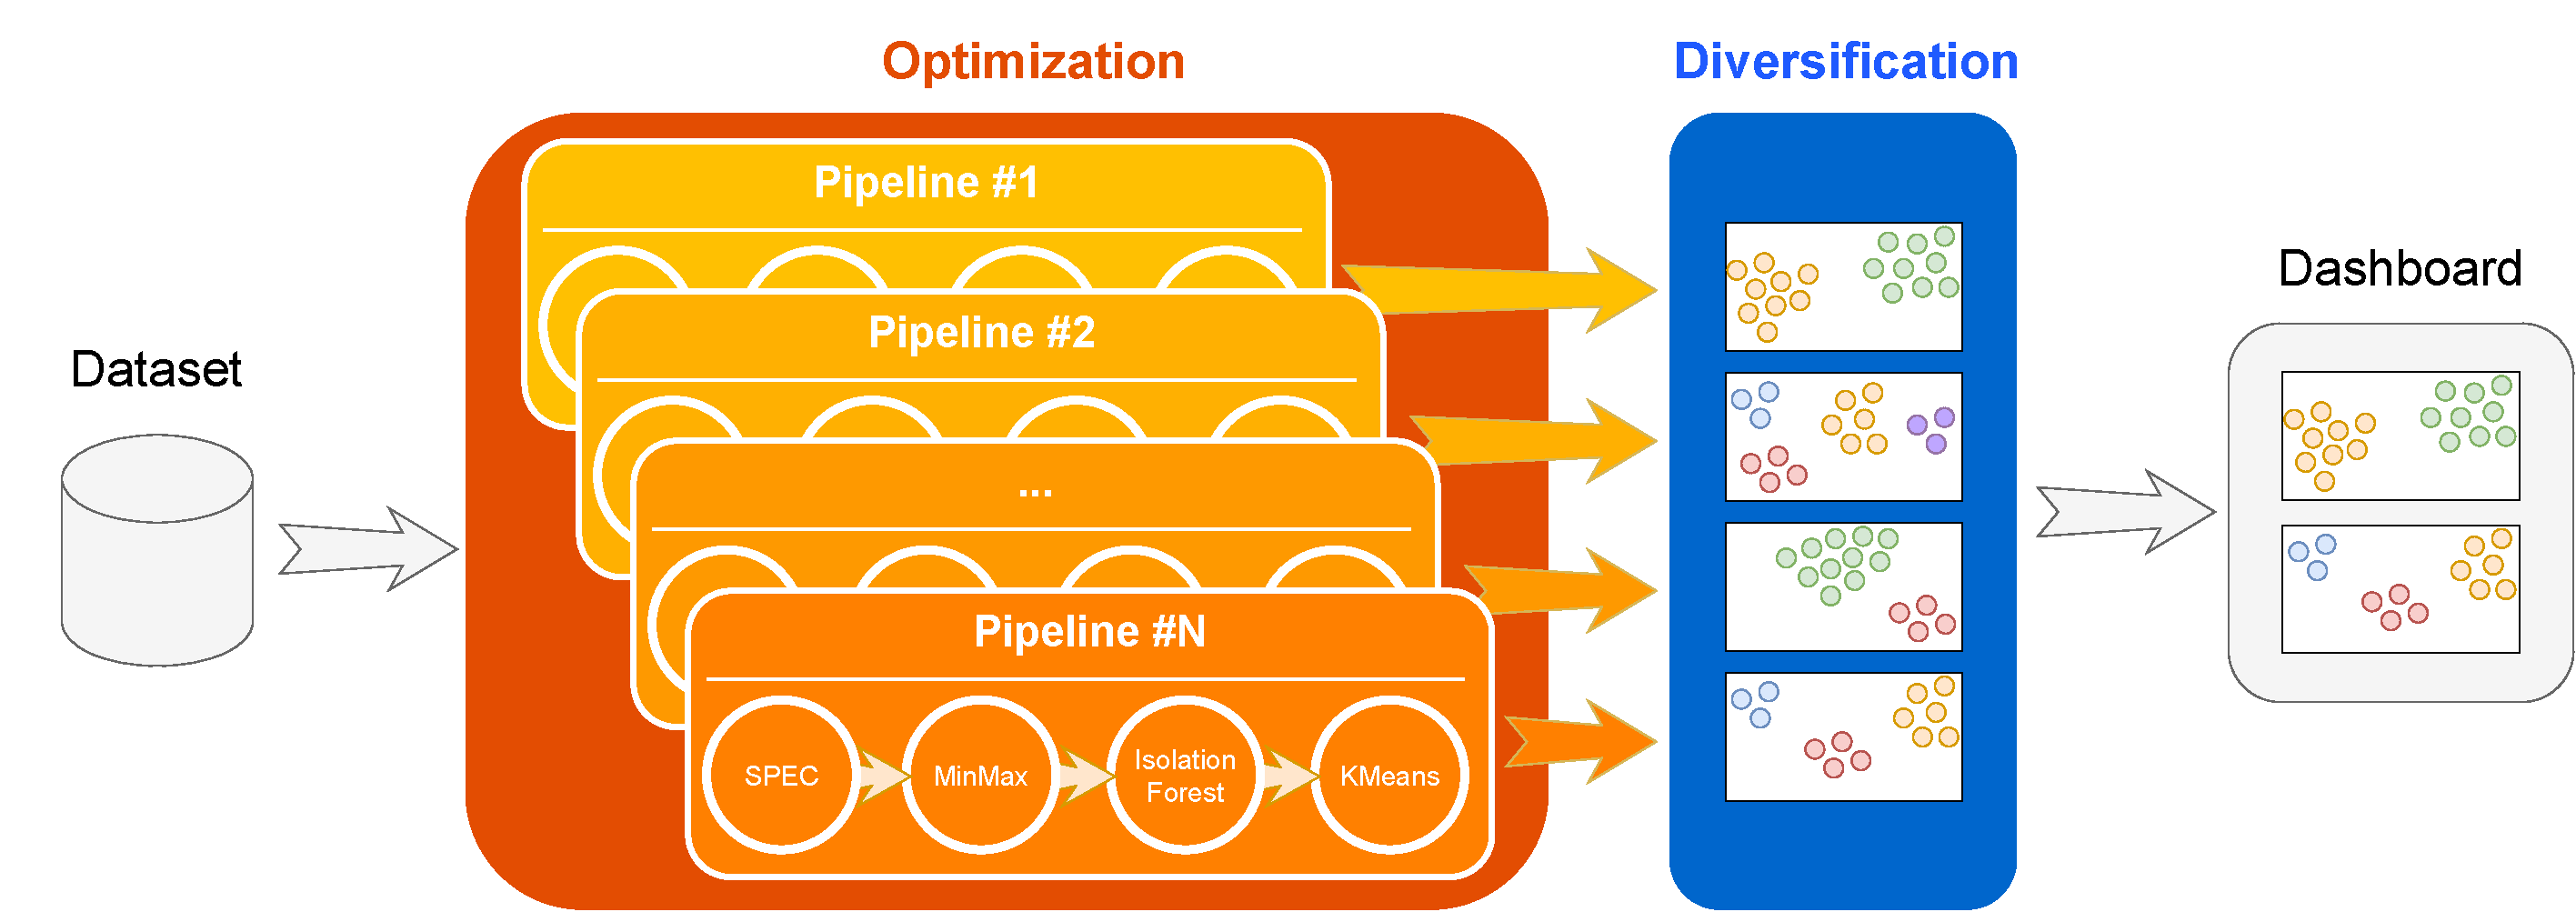
\includegraphics[scale=.26]{chapters/data-centric/unsupervised/img/approach.pdf}
    \caption{Overview of AutoClues.}
    \label{clustering-fig:overview}
\end{figure}

AutoClues aims at (i) tuning the whole ML pipeline and (ii) suggesting multiple clusterings to provide the data scientist different facets of the datasets. 
% by combining both model-based (AutoML) techniques and diversification.
%
In literature, these two problems are addressed through \textit{optimization} and \textit{diversification} techniques respectively.
\Cref{clustering-fig:overview} shows an overview of the architecture.
%
% !!!!!!!!!!!!! ALTERNATIVA
% AutoClues aims at tuning the whole ML pipeline and suggests multiple clusterings by combining both model-based (AutoML) techniques and diversification.
% \Cref{clustering-fig:overview} shows an overview of the architecture. In Section \Cref{clustering-ssec:formalization} we formalize the approach and in \Cref{clustering-sec:implementation} we delve into the implementation.

%\vspace{-0.3cm}
\subsection{Formalization}
\label{clustering-ssec:formalization}

% Intuitively, a pipeline is a sequence of steps where, at each step, an algorithm can be picked among several alternatives.

%
% Given the set of possible combinations  $\{P^{(1)}, \dots, P^{(n)}\}$ (i.e., different choices of algorithms per step), we define the associated hyperparameter spaces ${\Lambda^{(1)}, \dots, \Lambda^{(n)}}$ where each $\Lambda^{(i)}$ is the union of the hyperparameter spaces of the algorithms chosen in $P^{(i)}$.
%
% Let assume $D$ be a dataset and denote $\lambda \in \Lambda^{(i)}$ a hyperparameter configuration, then $\altmathcal{M}(P^{(i)}_{\lambda}, D)$ is the quality metric that evaluates the pipeline instance $P^{(i)}_{\lambda}$ on the dataset $D$.
% %
% Hence, the optimization problem can be formulated as:
\subsubsection{Optimization} We seek for the most ``correct'' pipeline.
A pipeline is a sequence of steps that process a dataset in order to return a clustering and, at each step, an algorithm can be picked among several alternatives.

More formally, a \textit{dataset} $D$ is a collection of $|D|$ data items that is characterized by a set of features $\altmathcal{F}$ (i.e., columns).
%
An \textit{Algorithm} $A$ is a function that transforms a dataset $D'$ into a new dataset $D''$ and has a set of (possibly empty) \textit{hyperparameters} that regulates its behavior.
%
Each hyperparameter has a domain, and the possible algorithm configurations are represented as the Cartesian product of all the hyperparameter domains, denoted with $\Lambda_A$.
%
We call \textit{algorithm instance} $\lambda_A \in \Lambda_A$ an (ordered) tuple in which each hyperparameter has been assigned with a value from its domain.
%
For instance, a clustering algorithm is KMeans and two tunable hyperparameters can be: the number of clusters $k \in \mathbb{N}^+$ and the maximum iterations $iter \in \mathbb{N}^+$. 
%
% Hence, $\Lambda_\textup{KMeans} = [2..12] \times \mathbb{N}^+$.
% An example of algorithm instance is $\lambda_\textup{KMeans} = (3, 10^3)$, where $k=3$ and $iter=10^3$.

A pipeline \textit{step} $S$ is a set of algorithms that can be selected as alternatives to carry out the step goal, including the possibility to return the dataset as-is through the ``Identity'' algorithm $I$.
%
The step domain is defined as $\Lambda_S = \Lambda_{A_1} \cupdot \ldots \cupdot \Lambda_{A_{|S|}}$, therefore the disjoint union of the domain of each algorithm\footnote{If an algorithm has no hyperparameters ($\Lambda_{A} = \varnothing$), we set a placeholder $\Lambda_{A} = \{ 1 \}$.}. $\lambda_{S}$ denotes the algorithm instance selected for the step.
%
% The $\cupdot$ combines all the algorithm domains while retaining their original membership (i.e., it is possible to distinguish each algorithm domain included in the step domain).
% \footnote{
% When $\Lambda_{A} = \varnothing$ (i.e., the algorithm has no hyperparameters), we set a placeholder $\Lambda_{A} = \{ 1 \}$.
% This is necessary to compute the step domain since the disjoint union of a non-empty set and an empty set would return the former.}
%.
% This is necessary to distinguish hyperparameters from different algorithms (e.g., $k$ is the number clusters in both KMeans and Agglomerative clustering algorithms).

A \textit{Pipeline} $P$ is a sequence of steps, its domain is the Cartesian Product of the step domains $\Lambda_P = \Lambda_{S_1} \times \ldots \times \Lambda_{S_{|P|}}$, and a \textit{pipeline instance} is an ordered tuple of algorithm instances $\lambda_P = (\lambda_{S_1}, \ldots, \lambda_{S_{|P|}}) \in \Lambda_P$.
The input of $\lambda_{A_i}$ is the output of $\lambda_{A_{i-1}}$ and the initial dataset $D$ is the input of $\lambda_{A_{1}}$.
In our use case, the last step is mandatory since it fulfills cluster analysis by returning a clustering.

A \textit{(crisp) Clustering} is a partition of the dataset into a set of (non-overlapping) clusters  $C=\{c_1, \ldots, c_{|C|}\}$ (i.e., groups of data items) by minimizing the distance of data items in the same cluster and maximizing the distance of different clusters. 
Given a pipeline domain $\Lambda_P$ and a dataset $D$, the optimal pipeline instance is 
\begin{equation}
\label{eq:optimization}
    \lambda_P^* = argmax_{\lambda_P \in \Lambda_P} rel(C)
\end{equation}
where $rel$ is a goodness metric for $C$ obtained by applying $\lambda_P$ on $D$.

\vspace{-0.3cm}
\subsubsection{Diversification} The process of returning a set of relevant and diverse solutions -- clusterings in our case -- is known as diversification, a multi-objective optimization problem that can be formulated as follows.
%
Let $\altmathcal{C}$ be the set of clusterings that have been previously explored in the pipeline optimization process (\Cref{eq:optimization}), then our goal is selecting a set of $\alpha$ clusterings $\altmathcal{C}^* \subseteq \altmathcal{C}$ maximizing a \textit{score} that represents a tradeoff between finding \textit{relevance} and \textit{diversity}.
%
\begin{align}\label{def:score}
&\altmathcal{C}^* = argmax_{\hat{\altmathcal{C}} \subseteq \altmathcal{C}, \alpha=|\hat{\altmathcal{C}}|} score(\beta, \hat{\altmathcal{C}})\\
&score(\beta, \hat{\altmathcal{C}}) = (1-\beta)~rel(\hat{\altmathcal{C}}) + \beta~div(\hat{\altmathcal{C}})
\end{align}
where $\beta \in [0.. 1]$ is the tradeoff parameter and
\begin{align}
rel(\hat{\altmathcal{C}}) &= (|\hat{\altmathcal{C}}|-1)\sum_{C \in \hat{\altmathcal{C}}} rel(C)
\label{def:rel}
\end{align}
\vspace{-1cm}
\begin{align}
div(\hat{\altmathcal{C}}) &= \sum_{C_i \in \hat{\altmathcal{C}}}~\sum_{C_j \in (\hat{\altmathcal{C}} \setminus C_i)} div(C_i, C_j)
\label{def:div}
\end{align}

\noindent $div(\hat{\altmathcal{C}})$ is the sum of pair-wise clustering diversity comparisons and $rel(\hat{\altmathcal{C}})$ is the sum of clustering relevance;
$rel(\hat{\altmathcal{C}})$ entails a multiplication factor $|\hat{\altmathcal{C}}|-1$ to make $rel(\hat{\altmathcal{C}})$ and $div(\hat{\altmathcal{C}})$ comparable.

% Relevance and diversity functions will be further discussed in the following.
% In our prototype, we set $\beta=0.7$ after empirical evaluation.

%\vspace{-0.2cm}
\subsection{Implementation}\label{clustering-sec:implementation}

\begin{table}[t]
    \centering
    \begin{tabular}{llcc}
        \hline
        Step     & Algorithm & \#Hyper. & $|\Lambda_A|$\\\hline
        Feature selection & SPEC \cite{zhao2007spectral} & 1 & $|\altmathcal{F}|-1$\\
         & WKMeans \cite{WKMeans} & 2 & $3 \cdot (|\altmathcal{F}|-1)$\\
         & Pearson Filtering & 1 & 10\\
        Normalization     & Standardization & 0 & 1\\
        & Robust Scaling & 3 & 12\\
        & MinMax & 0 & 1\\
        Outlier removal   & Local Outlier Factor \cite{breunig2000lof} & 1 & 3\\
        & Isolation Forest \cite{liu2012isolation} & 1 & 3\\
        %Cluster analysis  & KMeans \cite{arthur2006k} & $n \in [2.. \frac{|D|}{2}]$ \\
        Clustering  & KMeans \cite{arthur2006k} & 1 & $\sqrt{|D|}$\\
        & Agglomerative clustering  \cite{murtagh2017algorithms} & 1 & $\sqrt{|D|}$\\\hline
    \end{tabular}
    \vspace{0.2cm}
    \caption{Steps and algorithms optimized by AutoClues.}
    \label{clustering-tbl:processing}
\end{table}


\Cref{clustering-tbl:processing} reports the pipeline with steps, algorithms, and hyperparameters; AutoClues implementation can be found at \url{https://github.com/anonymous-pakdd-24/autoclues}.
The first step is \textit{Feature selection}. 
Since cluster analysis is particularly sensitive to non-informative and correlated features, we leverage algorithms from spectral family and based on the Pearson correlation, respectively. 
% Since cluster analysis is particularly sensitive to irrelevant features, this step aids in identifying the most informative ones.
% We leverage algorithms from the spectral family (SPEC and WKMeans), techniques that demonstrated to be effective in unsupervised tasks \cite{alelyani2018feature}, and based on the Pearson correlation.
Follows, \textit{Normalization} to adjust values on different scales and ensure that all the features contribute equally to the cluster formation.
Here, the literature has a considerable consensus on the well-known techniques such as Standardization, Robust scaling, and Min-max.
% Follows, \textit{Normalization} to adjust values on different scales and ensure that all the features contribute equally to the cluster formation.
% Here, the literature has a considerable consensus on the well-known techniques such as Standardization, Robust scaling, and Min-max that leverage statistical indicators; respectively: mean and standard deviation, median and quantile range, and max and min.
The last pre-processing step is \textit{Outlier Removal} for discarding any data points that are not representative of the cluster, we leverage Local Outlier Factor \cite{breunig2000lof} and and Isolation Forest \cite{liu2012isolation}.
% The last pre-processing step is \textit{Outlier Removal} for discarding any data points that are not representative of the cluster.
% Local Outlier Factor \cite{breunig2000lof} measures the anomaly score of each data item based on its local density deviation compared to its neighbors and Isolation Forest \cite{liu2012isolation} isolates elements by randomly selecting a feature and a split value within its minimum and maximum values.
Finally, the \textit{Clustering} step.
Since we focus on \textit{crisp spherical} clustering algorithms, we consider KMeans \cite{arthur2006k} and Agglomerative Clustering \cite{murtagh2017algorithms} with complete linkage.
% The former separates the data items into groups so that each of them has an equal variance, minimizing a criterion known as the inertia or within-cluster sum-of-squares. 
% The latter builds a hierarchy of clusters by merging smaller clusters into larger ones. 
As to the order of steps, in \cite{giovanelli2022data}, the authors reduce the combinations of the former steps; we further constrained the order of the steps by computing several experiments and observing the impact of different alternatives.
% Our implementation imports the algorithms from the sklearn Python library.
% While the algorithms can require the assignment of additional hyperparameters (e.g., the maximum number of iterations in KMeans), we reduce the pipeline domain by considering only the most influential.

\vspace{-0.4cm}
\subsubsection{Optimization}
To explore promising pipeline instances, rather than exhaustive or grid searches, we leverage Bayesian Optimization (BO) \cite{hutter2011sequential}.
%
BO is iterative: as it explores hyperparameter configurations, it progressively builds an accurate model of the domain to decide the next configuration to explore.
The exploration continues until a budget in terms of either iterations or time is reached.

Selecting the optimal pipeline instance requires the relevance metric (i.e., $rel(C)$) to evaluate the goodness of the retrieved clustering.
In AutoClues, such a metric is customizable.
%
Well-known metrics leveraged for spherical clustering are: the silhouette index (SIL) \cite{zhu2010clustering}, contrasting the average distance to elements in the same cluster with the average distance to elements in other clusters, and the Davies-Bouldin Index (DBI) \cite{dbi}, computing the average similarity between clusters by comparing it with the size of the clusters themselves.
% ; and the Calinski-Harabasz Index (CHI) \cite{chi}, which is the ratio of the sum of between-clusters dispersion and of within-cluster dispersion for all clusters (where dispersion is defined as the sum of distances squared).
%
However, clustering metrics show a bias toward lower dimensionalities i.e., yielding higher scores when fewer features are chosen \cite{lensen2017using,hancer2020new}. 
To overcome this issue, we employ t-SNE \cite{van2008visualizing} for projecting the clusterings into a latent 2D space. 
Then, we compute the chosen metric in this transformed space, thereby removing the bias and enabling a fair evaluation of the clusterings across diverse feature spaces.
% have different optimal feature subsets and different clustering solutions

During the optimization, we also store the computed pipeline instances since our goal is returning diverse and relevant clusterings.

\vspace{-0.4cm}
\subsubsection{Diversification}
% Implementing diversification in cluster analysis consists of evaluating the extent to which two clusterings differ from each other.
% This affects how the dashboard of returned clusterings looks like, ensuring the goal of returning different dataset facets.
% It is crucial to rely on a metric that goes beyond the mere identification of shared cluster membership among different clusterings but, instead, takes into account structural interrelationships within them.
Implementing diversification in cluster analysis involves assessing the extent to which two clusterings differ from each other, hence how the returned dashboard looks.
It is crucial to rely on a metric that considers not only shared cluster membership but also structural interrelationships within them.

Information theory introduces the concept of Mutual Information, quantifying the degree of dependence between two variables and, more specifically, Adjusted Mutual Information (AMI) allows for chance agreement\footnote{In statistics, it serves as a baseline for assessing the significance in random variations.}---providing more robust and meaningful measures.
When applied to cluster analysis, AMI $\in [0, 1]$ considers the labels assigned to data points within clusters, assuming higher values when the clusters in one partition align with those in another.
Since we need a diversity metric, we adapt the formula as in:
$$div(C_i, C_j) = 1- AMI(C_i, C_j)$$ 
where $C_i, C_j$ clusterings coming from different pipeline instances.

Finally, considering that the diversification problem is NP-hard, we compute it by exploiting the MMR heuristic solution \cite{vieira2011query} that selects the best-performing clustering and iteratively adds the clusterings that most diversify the outcome.

%\vspace{-0.2cm}
\section{Benchmark Generation and Empirical Evaluation}\label{clustering-sec:test}


\begin{table}[t]
    \centering
    \begin{tabular}{l|ccccccc|cccc}
    \hline
        \multirow{2}{*}{Dataset}& \multicolumn{7}{c|}{Characteristics} & \multicolumn{4}{c}{AutoClues Performance} \\
        & $|D|$ & $|\altmathcal{F}|$ & $|\altmathcal{C}|$ & $\sigma(D)$ & $\sigma(\altmathcal{F})$ & $SIL_N$ & $SIL_B$ & $SIL$ & $AMI$ & Score & Div. time (s) \\ \hline
         \texttt{syn1} & 2905 & 2  & 3 & 0.15  & 0.50  & 0.72 & 0.48 & 0.79 & 1.0 & 4.12 & \num{1.64e03} \\ 
        \texttt{syn2} & 264 & 5  & 3 & 0.25  & 0.20  & 0.64 & 0.4 & 0.7 & 0.83 & 4.76 & \num{1.74e02} \\ 
        \texttt{syn3} & 900 & 7  & 12 & 0.11  & 0.14  & 0.88 & 0.6 & 0.92 & 1.0 & 4.39 & \num{1.51e03} \\ 
        \texttt{syn4} & 1446 & 2  & 13 & 0.22  & 1.00  & 0.59 & 0.31 & 0.85 & 0.95 & 3.92 & \num{2.99e03} \\ 
        \texttt{syn5} & 1673 & 4  & 8 & 0.17  & 0.25  & 0.71 & 0.54 & 0.81 & 0.99 & 4.22 & \num{2.18e03} \\ 
        \texttt{syn6} & 2905 & 2  & 3 & 0.15  & 0.50  & 0.72 & 0.61 & 0.84 & 0.87 & 4.63 & \num{1.07e03} \\ 
        \texttt{syn7} & 264 & 5  & 3 & 0.25  & 0.20  & 0.64 & 0.41 & 0.72 & 0.86 & 3.78 & \num{1.67e02} \\ 
        \texttt{syn8} & 1639 & 8  & 21 & 0.13  & 0.00  & 0.87 & 0.69 & 0.91 & 1.0 & 4.45 & \num{3.13e03} \\ 
        \texttt{syn9} & 525 & 3  & 2 & 0.21  & 0.00  & 0.66 & 0.42 & 0.69 & 0.87 & 3.96 & \num{3.67e02} \\ 
        \texttt{syn10} & 1446 & 2  & 13 & 0.22  & 1.00  & 0.59 & 0.32 & 0.86 & 0.97 & 4.03 & \num{4.09e03} \\ 
        \texttt{syn11} & 4813 & 10  & 3 & 0.27  & 0.40  & 0.46 & 0.17 & 0.09 & 0.42 & 2.92 & \num{1.08e02} \\ 
        \texttt{syn12} & 2905 & 2  & 3 & 0.15  & 0.50  & 0.72 & 0.57 & 0.79 & 1.0 & 4.48 & \num{1.62e03} \\ 
        \texttt{syn13} & 264 & 5  & 3 & 0.25  & 0.20  & 0.64 & 0.4 & 0.74 & 0.89 & 4.37 & \num{2.75e02} \\ 
        \texttt{syn14} & 525 & 3  & 2 & 0.21  & 0.00  & 0.66 & 0.22 & 0.71 & 0.9 & 4.38 & \num{5.81e02} \\ 
        \texttt{syn15} & 2905 & 2  & 3 & 0.15  & 0.50  & 0.72 & 0.61 & 0.81 & 1.0 & 4.06 & \num{1.13e03} \\ 
        \texttt{syn16} & 264 & 5  & 3 & 0.25  & 0.20  & 0.64 & 0.49 & 0.7 & 0.88 & 3.45 & \num{1.84e02} \\ 
        \texttt{syn17} & 900 & 7  & 12 & 0.11  & 0.14  & 0.88 & 0.41 & 0.92 & 1.0 & 4.62 & \num{1.45e03} \\ 
        \texttt{syn18} & 525 & 3  & 2 & 0.21  & 0.00  & 0.66 & 0.3 & 0.69 & 0.84 & 4.34 & \num{2.85e02} \\ 
        \texttt{syn19} & 2905 & 2  & 3 & 0.15  & 0.50  & 0.72 & 0.53 & 0.86 & 0.87 & 4.79 & \num{1.28e03} \\ 
        \texttt{syn20} & 264 & 5 & 3 & 0.25 & 0.20 & 0.64 & 0.44 & 0.7 & 0.88 & 3.74 & \num{2.13e02} \\ \hline
    \end{tabular}
    \vspace{0.2cm}
    \caption{Dataset characteristics and performance achieved by AutoClues.}
    \label{clustering-tbl:synthetic}
\end{table}



% Cluster analysis faces notably limited availability of benchmarks, i.e. suites of datasets that enable fair comparisons among different approaches.
% Given the numerous families of clustering (e.g., crisp, fuzzy) and corresponding cluster shapes (e.g., spherical, worm), existing benchmarks \cite{ClusteringDatasets,gagolewski2022framework,thrun2020clustering} solely cover the scenarios for which they were designed.
% In our use case, no benchmarks are available and approaches borrow and report performance on datasets from supervised tasks.
% Yet, with no guarantees on the underlying clusters' shape, comprehensive evaluations remain rather difficult. 
% \mg{Io qui non partirei da dal benchmark generator ma da un commento genererico dato che il generatore è il contributo meno importante ed incidentale. possiamo definire i nostri obiettivi di test e dire che non ha senso farlo solo su dataset reali perchè il nostro sistema utilizza k-means e quindi è opportuno cercare cluster sferici. Dato che dataset con cluster sferici non ci sono abbiamo fatto il generatore}

Evaluation in cluster analysis consists of assessing the approach performance in finding well-separated clusters and -- if available -- their alignment with a hypothetical ground truth.
It is crucial to test on datasets that conform with the leveraged clustering algorithms, e.g., in our case, containing crisp spherical clusters.
Yet, there is a lack of benchmarks (i.e., suites of datasets for fair comparisons) and the few available \cite{ClusteringDatasets,gagolewski2022framework,thrun2020clustering} are tailored to their specific scenarios.
This translates into approaches relying upon datasets from supervised tasks, with no guarantees on the underlying clusters' shape.


% Cluster analysis lacks benchmark availability i.e., suites of datasets for fair comparisons, mainly due to the large number of clustering families (e.g., crisp, fuzzy) and cluster shapes (e.g., spherical, worm). Existing benchmarks \cite{ClusteringDatasets,gagolewski2022framework,thrun2020clustering} are tailored to their specific scenarios, leading cases as ours to the reliance on datasets from supervised tasks. 
% Yet, with no guarantees on the underlying clusters' shape, comprehensive evaluations remain challenging.

In \Cref{clustering-ssec:benchmark}, we introduce a benchmarking generator and a suite of synthetic datasets. In \Cref{clustering-ssec:effectiveness}, we leverage such a suite to assess the effectiveness and efficiency of AutoClues.
Finally, in \Cref{clustering-ssec:comparison}, we rely on real datasets to provide a comparison against other approaches in the literature.

\vspace{-0.2cm}
\subsection{Benchmark Generation}
\label{clustering-ssec:benchmark}
% \mg{Storytelling: generiamo dei cluster naturali fissandone le caratteristiche ..... e poi li nascondiamo (to blur) aggiungendo un insieme di deformazioni ..... di cui governiamo le caratteristiche. $SIL_N$ è la complessità dei cluster naturali $SIL_B$ è la complessità dei cluster blurred.}
The synthetic benchmarking generator is available at \url{https:/github.com/anonymous-pakdd-24/clustering_benchmarking}.
We create datasets of $|D|$ instances, defining $|C|$ natural iper-spherical clusters in a space of $|\altmathcal{F}|$ features.
Then, we blur such clusters by posing common challenges faced by clustering algorithms. 
This includes noise on instances $\sigma(D)$, such as the presence of outliers, and
noise on features $\sigma(F)$, such as irrelevant, correlated, or distorted features.
% Our benchmark generation is based on well-known dimensions that characterize the dataset complexity. 
% One the one hand, some of these are intrinsic such as cardinality i.e., the number of instances $|D|$; 
% which affects the efficiency of most algorithms; 
% dimensionality i.e., the number of features $|\altmathcal{F}|$; 
% which has a significant impact on distance measures; 
% the number of natural clusters $|C|$.
% influencing cohesion and separability within the one known partinioning---among the potential ones. 
% On the other hand, we apply noise with a certain degree to pose common challenges faced by clustering algorithms. This includes noise on instances $\sigma(D)$, such as the presence of outliers, and
% i.e., anomalous data which deviate to typical or expected patterns within the dataset;
% noise on features $\sigma(F)$, such as irrelevant, correlated, or distorted features.
% that complicate the task by distorting the feature space,  resulting in a dataset that is more skewed or less representative of the underlying patterns. 

%\vspace{-0.03cm}
To obtain datasets with different characteristics, we set boundaries for each of these dimensions and sample within them according to the Sobol sequence \cite{sobol1967distribution}, a quasi-random low-discrepancy search converging to an equi-distributed coverage. 
In particular, the defined boundaries are: $|D|$ between $100$ and $5000$, $|F|$ between $2$ and $10$, $|C|$ between $2$ and $\sqrt{|D|}$, $\sigma(D)$ between $0.1$ and $0.3$, and $\sigma(F)$ between $0$ and $1$.
% Subsequently, datasets can be sampled within these predefined ranges.
\Cref{clustering-tbl:synthetic} provides a suite of $20$ synthetic datasets. 

%\vspace{-0.03cm}
Dataset complexity can be examined via the silhouette $SIL \in [0, 1]$, the higher the simpler. 
$SIL_N$ measures the cohesion and separability of the natural clusters $C$ in their original feature space, while  $SIL_B$ measures the silhouette of blurred clusters (i.e. after introducing noise ($\sigma$)).
The former $SIL_N$ indicates the presence of well-separated clusters.
With the first quartile $Q1=0.64$, median $Q2=0.66$, and third quartile $Q3=0.72$, we observe that 25\% of datasets are complex already at this stage. 
The latter $SIL_B$ registers significantly lower values: \texttt{syn11} emerges as an especially complex dataset with $SIL_B=0.17$ but, overall, we confirm the presence of a good distribution between more and less challenging datasets: $Q1 = 0.36$, $Q2 = 0.43$, and $Q3 = 0.55$.
% Lastly, $SIL_{\Delta} = SIL_B - SIL_N$ reports the difference between $SIL_N$ and $SIL_B$, highlighting critical datasets such as syn14 and syn17 with drops of $0.44$ and $0.47$ respectively.

\vspace{-0.2cm}
\subsection{Effectiveness and efficiency}
\label{clustering-ssec:effectiveness}


We test AutoClues on the suite of generated synthetic datasets.
For the optimization, we adopted the silhouette $SIL$ index as a relevance objective metric and a budget of $7200$ second ($2$ hours); for the diversification we set $\alpha=3$ and $\beta=0.5$, resulting in a dashboard of $3$ clusterings where relevance and diversity are weighted equally.
Tests are run on a single core of an Intel Core i7 machine at $3.20$ GHz and $64$ GB of main memory.
%
Given an AutoClues dashboard, \Cref{clustering-tbl:synthetic} provides
% the achieved performance according to 
the maximum $SIL\in [0, 1]$ as the cohesion of the found clusters and the maximum $AMI \in [0, 1]$ as the alignment with the natural ones. Besides, we report the dashboard score of \Cref{def:score}, summarizing the overall relevance and diversity in the dashboard, and the computation time (in seconds) spent during the diversification process. 
% \mg{l'inglese è un po' contorto}

\vspace{-0.5cm}
\subsubsection{Effectiveness}\label{sssec:effectiveness}
% \mg{ Fare notarare che $SIL > SIL_N$ perchè AutoClues può eliminare dei punti (dei cluster naturali) che considera di rumore determinando quindi dei cluster più compatti}
The achieved silhouette not only shows AutoClues' ability to find particularly well-separated clusters in 19 cases out of 20, but it also demonstrates to overcome the silhouette of natural clusters $SIL_N$. 
% \mg{ma nei natural cluster non ci sono outlier. Meglio dire silhouette of natural clusters }
This is achieved through data pre-processing such as projecting natural clusters into more compact feature subsets and mitigating potential noise.
% , such as outliers.
The only exception is \texttt{syn11}, a dataset already highlighted as critical for both intrinsic characteristics and noise applied. 
% Observed quartile values of $SIL$ are reported: $Q1=0.71$, $Q2=0.79$, and $Q3=0.85$.
Besides, quartile values of $AMI$ ($Q1=0.87$, $Q2=0.9$, $Q3=1$) confirm a strong agreement between retrieved and natural clusters. 
% Aside from \texttt{syn11} that achieves $0.42$, AutoClues achieved at least $AMI=0.83$ in each dataset, with 25\% in which perfectly match the natural clusters ($AMI=1$). Overall, $Q1=0.87$, $Q2=0.9$, and $Q3=1$.

As to the dashboard, considering the experimental setting ($\alpha=3$, $\beta=0.5$,  $rel, div \in [0, 1]$), the score is bounded in $[0, 6]$.
% As to the dashboard score, this is bounded in highlights the impacts of both relevance \textit{rel} (\Cref{def:rel}) and diversification \textit{div} (\Cref{def:div}).
% Considering the experimental setting ($\alpha=3$, $\beta=0.5$,  $rel, div \in [0, 1]$), the score is bounded in $[0, 6]$.
% \mg{trade-off e complimentary piuttosto, 3 e 4 sono già buoni, noi abbiamo in media 4.2}
% Notably, given the low probability of both \textit{rel} and \textit{div} metrics simultaneously taking on extreme values (e.g., $1$), scoring values at the boundaries are particularly unlike to occur (e.g., $6$).
Notably, given the inherent trade-off relationship between \textit{rel} and \textit{div} in the context of a diversification problem, it is noteworthy that scores at the boundaries are less likely to manifest,
with values around $4$ already acknowledged as high-quality \cite{vieira2011query}.
Analogously, quartile values of the score ($Q1=4$, $Q2=4.34$, $Q3=4.47$) confirm Autoclues' ability to find relevant and diverse clusterings.
% to $SIL$ and $AMI$, we observe good performance. 
% Apart from \texttt{syn11},
%demonstrates again to be the most difficult dataset with a dashboard score of $2.92$.
% As to the remaining, 
% we observe quartile values of $Q1=4$, $Q2=4.34$, and $Q3=4.47$.

\vspace{-0.5cm}
\subsubsection{Efficiency}\label{sssec:efficiency}
\Cref{clustering-tbl:synthetic} reports the computation time for diversification, when the optimization budget is set to 2 hours.
We can observe 25\% of datasets compute the dashboard in less than $Q1=\num{2.44e02}$ seconds ($4$ minutes), $50\%$ in less than $Q2=\num{1.07e03}$ seconds ($18$ minutes), and $75\%$ in less than $Q3=\num{1.56e03}$ seconds ($26$ minutes).
Besides, reducing the optimization budget leads to a decrease in diversification time, as fewer clusterings are evaluated, while the overall performance is largely maintained.

\begin{figure}[t]
    \centering
    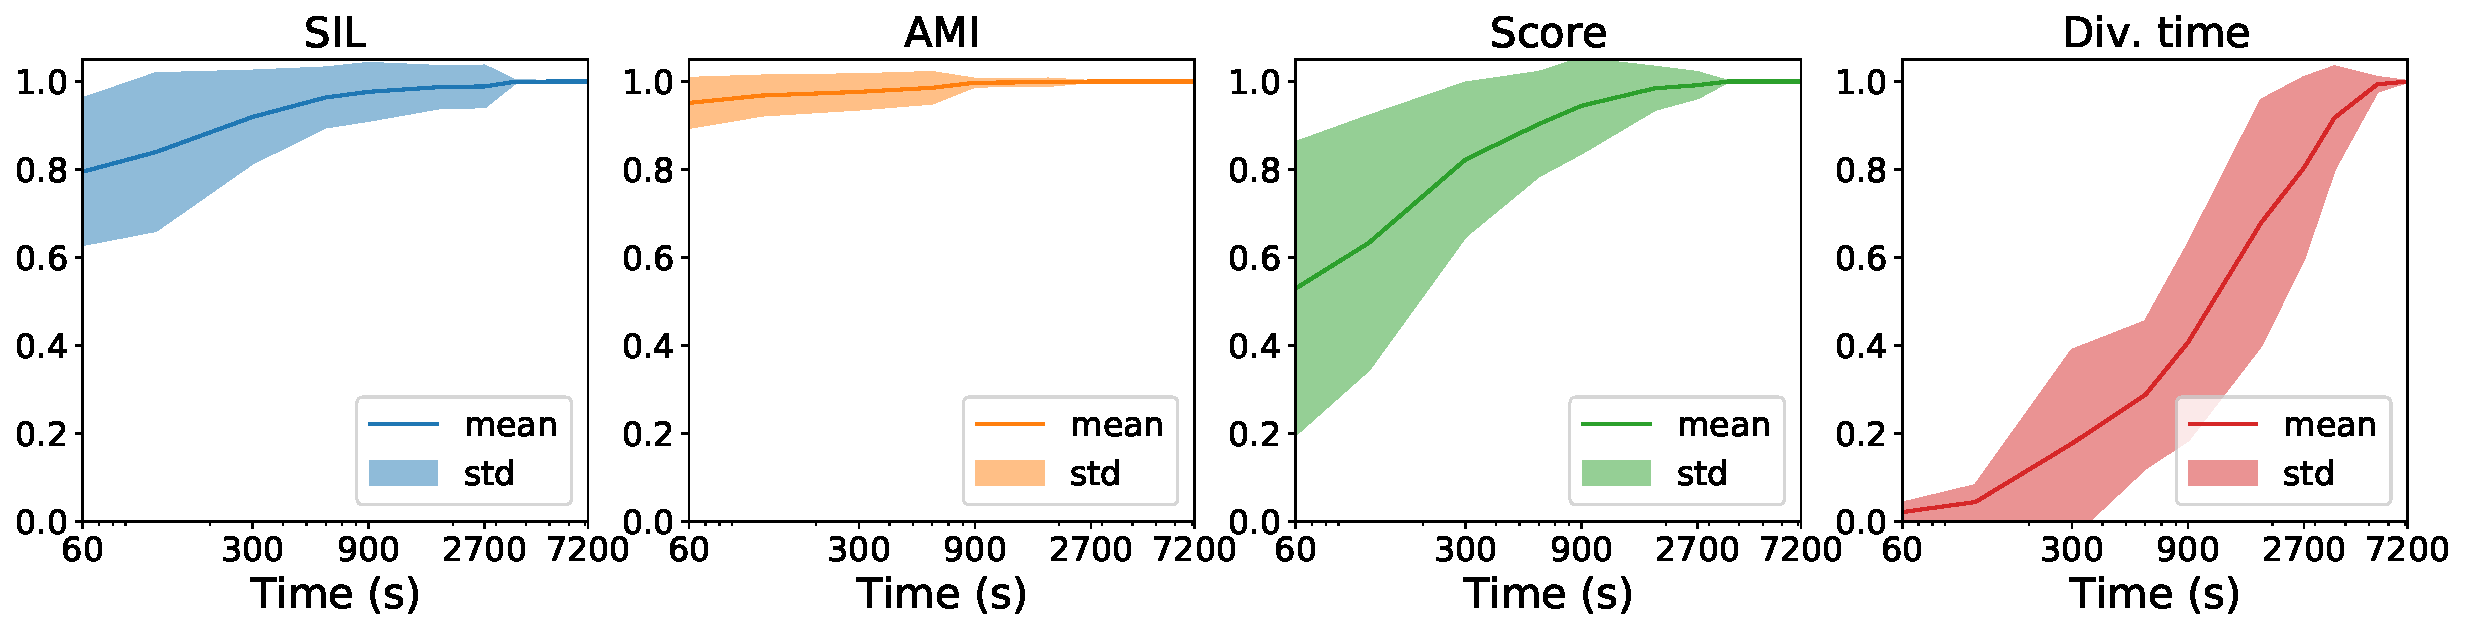
\includegraphics[scale=.3]{chapters/data-centric/unsupervised/img/all.pdf}
    \caption{AutoClues convergence through time (in log scale).}
    \label{clustering-fig:convergence}
\end{figure}

\Cref{clustering-fig:convergence} shows how AutoClues converges to the values reported in \Cref{clustering-tbl:synthetic}.
Dashboards are generated at different snapshots during the $2$-hour optimization process, and the same metrics are computed: $SIL$, $AMI$, dashboard score, and diversification time.
We summarize the information by plotting the mean and standard deviation among the whole suite, the convergence is quantified as a progress ratio relative to the final achieved performance.
%
Notably, the optimization time is illustrated in a logarithmic scale, which is already evidence of fast convergence.
After $60$ seconds of optimization, we have clusterings with $SIL$ and $AMI$ as good as $80\%$ and $95\%$ of the optimal and a dashboard almost $60\%$ of the final within a negligible diversification time---roughly $2\%$ of the total, $30$ seconds on average.
% Indeed, clusterings with $SIL$ as good as $80\%$ of the optimal one and $AMI$ as good as $95\%$ of the optimal one are on average achieved already after $60$ seconds of computation, and in the worst case not less than $60\%$ and $90\%$ respectively. 
% An average of $90\%$ of $SIL$ and $97\%$ of $AMI$ is registered within $300$ seconds ($5$ minutes), $95\%$ of $SIL$ and $100\%$ of $AMI$ within $900$ seconds ($15$ minutes), and $SIL$ reaches $100\%$ within $2700$ seconds ($45$ minutes).
%
% As to the dashboard,
% after $60$ seconds of optimization, we have almost $60\%$ of the final dashboard within a negligible diversification time---roughly $2\%$ of the total, $30$ seconds on average.
Within $300$ seconds of optimization, an average of $90\%$ of $SIL$, $97\%$ of $AMI$, and $75\%$ of the dashboard score are registered with a diversification cost of $10\%$---on average, $1$ minute and half.
The trends of $SIL$ and $AMI$ saturated $100\%$ right afterward, while both dashboard score and cost increase linearly until $900$ seconds of optimization, in which the dashboard achieves $90\%$ of its score within a cost of $30\%$---$5$ minutes on average.
After such a threshold, improvements in the score are not considered worth it for the computation cost.
This is due to the increasing number of available solutions that have to be evaluated during the diversification, while relevant and diverse clusterings are already present in the dashboard.

\vspace{-0.2cm}
\subsection{Comparison}\label{clustering-ssec:comparison}

% \begin{table}[t]
%     \centering
%         \begin{tabular}{l|ccc}
%             \hline
%             \multirow{2}{*}{Dataset} & \multirow{2}{*}{$|D|$} & \multirow{2}{*}{$|\altmathcal{F}|$} & \multirow{2}{*}{$|C|$} \\ 
%             & & & \\ \hline
%             blood & 748 & 4 & 2 \\
%             breast & 106 & 9 & 6 \\
%             ecoli & 327 & 7 & 5 \\
%             iris & 150 & 4 & 3 \\
%             seeds & 210 & 7 & 3 \\
%             thyroid & 215 & 5 & 3 \\
%             vehicle & 846 & 18 & 4 \\
%             wine & 178 & 13 & 3 \\ \hline
%         \end{tabular}
%         \quad
%     \begin{tabular}{l|cc|cc|cc|cc}
%         \hline
%         \multirow{2}{*}{Dataset} & \multicolumn{2}{c|}{MOGA} & \multicolumn{2}{c|}{MODE-cf} & \multicolumn{2}{c|}{MALSS} & \multicolumn{2}{c}{AutoClues} \\
%         & \multicolumn{1}{c|}{SIL} & DBI & \multicolumn{1}{c|}{SIL} & DBI & \multicolumn{1}{c|}{SIL} & DBI & \multicolumn{1}{c|}{SIL} & DBI \\ \hline
%         blood & - & - & - & - & 0.73 & 0.3 & 1 & f \\ 
%         breast & - & - & - & 0.7 & 0.16 & 1.6 & 0.60 & 0.54 \\ 
%         ecoli & - & - & - & 0.92 & 0.72 & 0.35 & 0.46 & 0.84 \\ 
%         iris & - & 0.39 & - & 0.67 & 0.57 & 0.6 & 0.71 & 0.38 \\ 
%         seeds & - & - & - & - & 0.45 & 0.8 & 0.37 & f \\ 
%         thyroid & - & - & - & - & 0.6 & 0.64 & 0.92 & f \\ 
%         vehicle & - & - & - & - & 0.61 & 0.6 & 0.72 & f \\ 
%         wine & - & 0.77 & - & 1.22 & 0.28 & 1.4 & 0.38 & 1.01 \\ \hline
%     \end{tabular}
%     \caption{Comparison with other approaches in the literature.}
%     \label{clustering-tbl:comparison}
% \end{table}

% \begin{table}[t]
%     \centering
%     \centering
%     \begin{tabular}{l|ccc|cc|cc|cc|cc}
%     \hline
%         \multirow{3}{*}{Dataset} & \multicolumn{3}{c|}{Characteristics} & \multicolumn{8}{c}{Performance} \\
%         & \multirow{2}{*}{$|D|$} & \multirow{2}{*}{$|\altmathcal{F}|$} & \multirow{2}{*}{$|C|$} & \multicolumn{2}{c|}{MOGA \cite{dutta2013}} & \multicolumn{2}{c|}{MODE-cf \cite{hancer2020new}} & \multicolumn{2}{c|}{MALSS \cite{Kamoshida2020}} & \multicolumn{2}{c}{AutoClues} \\ 
%         & & & & \multicolumn{1}{c|}{SIL} & DBI & \multicolumn{1}{c|}{SIL} & DBI & \multicolumn{1}{c|}{SIL} & DBI & \multicolumn{1}{c|}{SIL} & DBI \\ \hline
%         Blood-transfusion & 748 & 4 & 2 & - & - & - & - & 0.73 & 0.3 & 1 & 0 \\ 
%         Breast-tissue & 106 & 9 & 6 & - & - & - & 0.7 & 0.16 & 1.6 & 0.60 & 0.54 \\ 
%         Ecoli & 327 & 7 & 5 & - & - & - & 0.92 & 0.72 & 0.35 & 0.46 & 0.84 \\ 
%         Iris & 150 & 4 & 3 & - & 0.39 & - & 0.67 & 0.57 & 0.6 & 0.71 & 0.38 \\ 
%         Seeds & 210 & 7 & 3 & - & - & - & - & 0.45 & 0.8 & 0.37 & 0.4 \\ 
%         Thyroid-new & 215 & 5 & 3 & - & - & - & - & 0.6 & 0.64 & 0.92 & 0.2 \\ 
%         Vehicle & 846 & 18 & 4 & - & - & - & - & 0.61 & 0.6 & 0.72 & 0.15 \\ 
%         Wine & 178 & 13 & 3 & - & 0.77 & - & 1.22 & 0.28 & 1.4 & 0.38 & 1.01 \\ \hline
%     \end{tabular}
%     \caption{Comparison with other approaches in the literature.}
%     \label{clustering-tbl:comparison}
% \end{table}


\begin{table}[t]
    \centering
    \begin{tabular}{l|ccc|cccc|cc}
    \hline
        \multirow{3}{*}{Dataset} & \multicolumn{3}{c|}{Characteristics} & \multicolumn{6}{c}{Performance} \\
        & \multirow{2}{*}{$|D|$} & \multirow{2}{*}{$|\altmathcal{F}|$} & \multirow{2}{*}{$|C|$} & \multicolumn{4}{c|}{DBI $\downarrow$} & \multicolumn{2}{c}{SIL $\uparrow$} \\
        & & & & \multicolumn{1}{c}{MOGA} & \multicolumn{1}{c}{MODE-cf} & \multicolumn{1}{c}{MALSS} & \multicolumn{1}{c|}{AutoClues} & \multicolumn{1}{c}{MALSS} & \multicolumn{1}{c}{AutoClues} \\ \hline
        \texttt{blood} & 748 & 4 & 2 & - & - & 0.3 & \textbf{0} & 0.73 & \textbf{1} \\ 
        \texttt{breast} & 106 & 9 & 6 & - & 0.7 & 1.6 & \textbf{0.54} & 0.16 & \textbf{0.60} \\ 
        \texttt{ecoli} & 327 & 7 & 5 & - & 0.92 & \textbf{0.35} & 0.46 & \textbf{0.72} & 0.46 \\ 
        \texttt{iris} & 150 & 4 & 3 & 0.39 & 0.67 & 0.6 & \textbf{0.38} & 0.57 & \textbf{0.71} \\
        \texttt{seeds} & 210 & 7 & 3 & - & - & 0.8 & \textbf{0.4} & \textbf{0.45} & 0.37 \\
        \texttt{thyroid} & 215 & 5 & 3 & - & - & 0.64 & \textbf{0.2} & 0.6 & \textbf{0.92} \\ 
        \texttt{vehicle} & 846 & 18 & 4 & - & - & 0.6 & \textbf{0.15} & 0.61 & \textbf{0.72} \\ 
        \texttt{wine} & 178 & 13 & 3 & \textbf{0.77} & 1.22 & 1.4 & 1.01 & 0.28 & \textbf{0.38} \\ \hline
    \end{tabular}
    \vspace{0.2cm}
    \caption{Comparison with other approaches in the literature.}
    \label{clustering-tbl:comparison}
\end{table}


We compare AutoClues with state-of-the-art approaches in the literature against real datasets, considered as standard benchmarks.
We selected the ones that provided either the performance on classification datasets (MOGA \cite{dutta2013}, MODE-cf \cite{hancer2020new}) or code for reproducibility (MALSS \cite{Kamoshida2020}).
The former two approaches are evolutionary algorithms, and the latter is a general-purpose AutoML tool.
Note that all these approaches do not provide a dashboard of clusterings, but only the best performing one.
Thus, for a fair comparison, we set $\alpha=1$ to return the best clustering as well and we adopt as relevance the same metric used in the competing approaches.
MOGA and MODE-cf measure performance solely through the Davies–Bouldin Index ($DBI$ \cite{dbi}, the less the better),
% The minimum score is 0 with lower values indicating better clustering.
MALLS also provides $SIL$ (the higher the better).

\Cref{clustering-tbl:comparison} shows that AutoClues outperforms the reported approaches in 6 out of 8 datasets.
According to $DBI$, MALSS achieves better performance on \texttt{seeds}, while MOGA on \texttt{wine}.
As to $SIL$, MALSS is slightly more performant in \texttt{ecoli} and \texttt{seeds}.
Yet, this is due to the fact that such approaches support the computation of non-spherical clusterings while they are not currently included in AutoClues.
Indeed, if we constraint MALSS to compute spherical clusters only, we observe a $DBI$ value of $0.79$ for \texttt{ecoli} while AutoClues achieves $0.46$ (the less the better).
As to $SIL$, MALLS achieves $0.4$ and $0.45$ for \texttt{ecoli} and \texttt{seeds} respectively; AutoClues outperforms on \texttt{ecoli} with $SIL=0.46$ and confirms the previous result on \texttt{seeds} with $SIL=0.37$.

% Overall, these results confirm that optimizing pre-processing boosts the performance of AutoClues. \mg{questa è la conclusione principale}

\vspace{-0.2cm}
\section{Conclusion and Future Work}\label{clustering-sec:conclusion}
We introduced AutoClues, an end-to-end cluster analysis approach that leverages AutoML techniques to provide a diverse and relevant dashboard of clusterings. Our findings demonstrate that optimizing pre-processing significantly enhances performance, allowing AutoClues to overcome current state-of-the-art approaches. For future research, we plan to explore (i) meta-learning approaches to identify more effective pre-processing steps, (ii) integrating human feedback in the loop, and (iii) providing automatic explanations for the retrieved dashboard.

% We introduced AutoClues, an end-to-end approach for cluster analysis that explores ML pipelines through AutoML techniques and retrieves a dashboard of relevant and diverse clusterings---i.e., facets of the dataset.
% Results confirm that optimizing pre-processing boosts performance, enabling AutoClues to overcome state-of-the-art approaches. 
% AutoClues's pipeline exploration, carried out using AutoML techniques, overcomes the state-of-the-art approaches for clustering analysis since it improves the optimization of the thorough clustering pipeline. 
% As future research directions, we plan to (i) identify with meta-learning approaches which pre-processing steps are more effective to bias both optimization and diversification, (ii) include the human in the loop (e.g., learning a measure of interest by examples), and (iii) carry out an automated explanation process that describes the dashboard (i.e., which are the main insights of the facets retrieved by AutoClues).

